%# -*- coding: utf-8-unix -*-
%%==================================================
%% 04_results.tex % 4k
%%==================================================


\chapter{实验结果与分析}

\label{chap:results}

\section{功耗曲线}

按照在 \ref{sec:collect} 节所述的流程,在密码算法电路运行时,采集其功耗,并记录存储到计算机上。本次实验一共采集了 100 万条功耗曲线,实际用到的为前 2 万条。密码算法跑在普通的 FPGA 上,这里的功耗值对应的具体物理量,实际上是电路电源线上的总电流。 \cite{zuc_fpga} \cite{zuc_fpga_en}

由于我们的攻击针对的是 ZUC 算法的初始化阶段,因此只储存了初始化阶段的功耗点。初始化阶段一共有 32 轮,这里只记录了前 27 轮,不过这也已经足够我们使用了。

\vspace*{\baselineskip}

图 \ref{fig:traces} 展示了第 1、20、200、2000 和 20000 条功耗曲线的波形。

从图中可以得到这样一些信息:

\begin{enumerate}
    \item \textbf{时钟频率以及电路运行状况稳定。}\\
    图中的曲线在各个时间点处的峰值基本对齐,说明时钟频率非常稳定,并且每次运行算法所花费的时间几乎是相同的。从抽取的曲线来看,波形也几乎一致。这意味着我们可以免去对齐曲线这部分预处理的工作,降低了工作量,清晰的轮廓也从侧面反映了采集得到的功耗曲线质量较高。因此得到这样的曲线是非常令人满意的。
    \item \textbf{采集到的曲线包含了密钥装载阶段和前 27 轮初始化。}\\
    前面一段持续的高功耗,应该是算法电路的启动,以及相关数据载入内存并交由控制器的部分,其中的一个尖峰,可能是密钥装载的阶段。之后可以看到 27 个特征相似的波形,毫无疑问,这是算法中初始化阶段的 27 轮循环操作。图中的尖峰特征还是非常明显的,然而这并不代表一定会有密钥信息的泄露。诚然,在很多情况下,功耗的尖峰和明显的起伏,很可能是泄露点,但是具体的泄露位置以及泄露程度,还是需要后续的分析才能确定。
\end{enumerate}

\begin{figure}[htbp]
    \centering

    \begin{subfigure}{1.0\textwidth}
        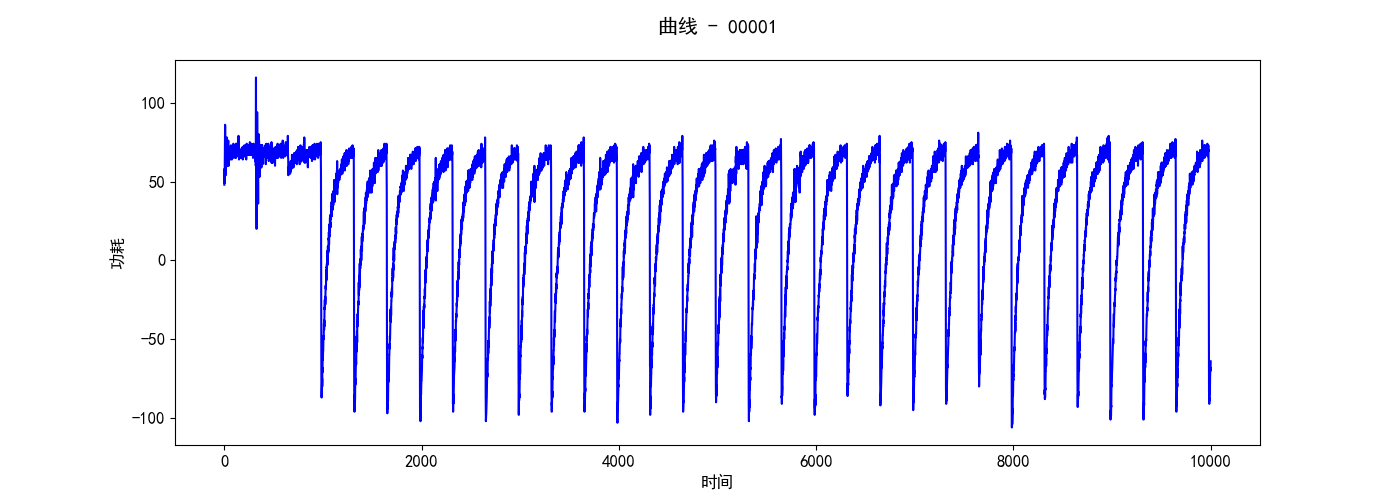
\includegraphics[height=.17\textheight, width=1.0\textwidth]{../images/trace_00001.png}
        % \caption{第 00001 条功耗曲线}
    \end{subfigure}
    \begin{subfigure}{1.0\textwidth}
        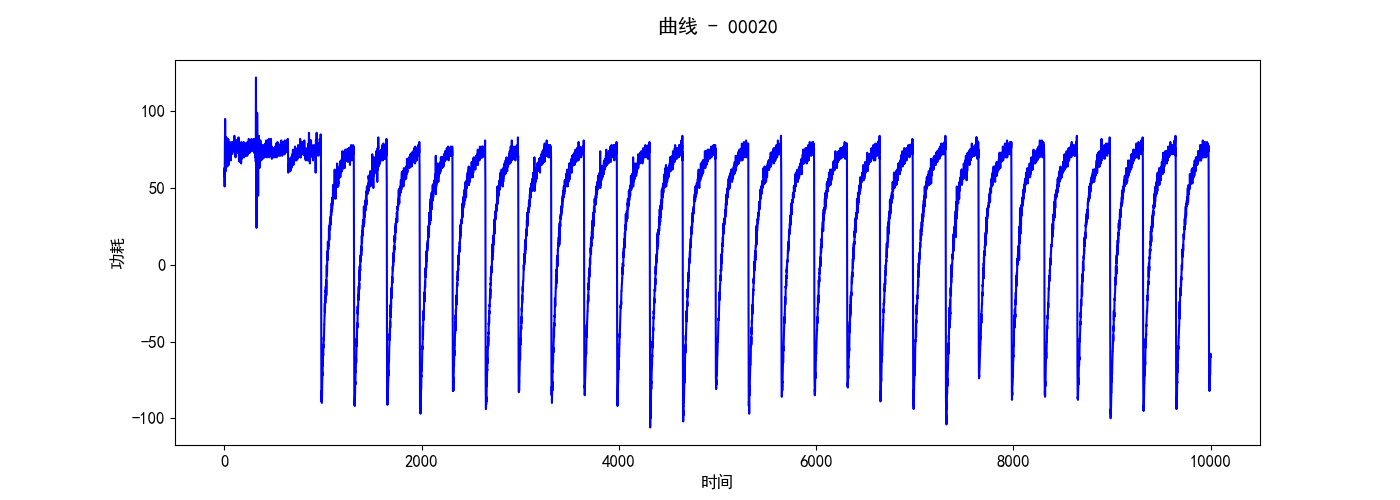
\includegraphics[height=.17\textheight, width=1.0\textwidth]{../images/trace_00020.png}
        % \caption{第 00020 条功耗曲线}
    \end{subfigure}
    \begin{subfigure}{1.0\textwidth}
        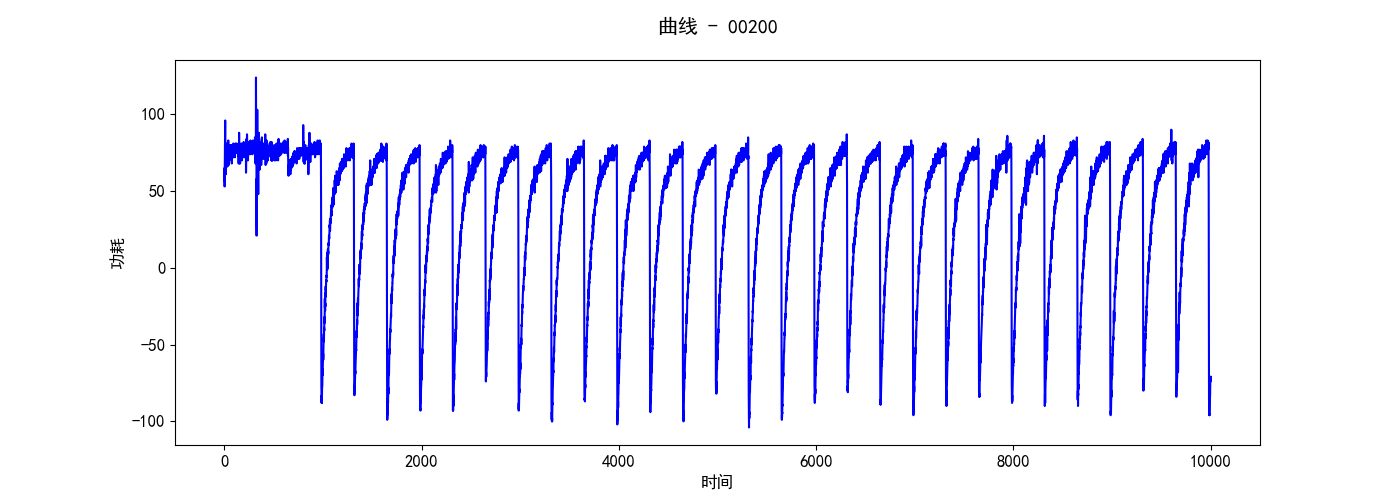
\includegraphics[height=.17\textheight, width=1.0\textwidth]{../images/trace_00200.png}
        % \caption{第 00200 条功耗曲线}
    \end{subfigure}
    \begin{subfigure}{1.0\textwidth}
        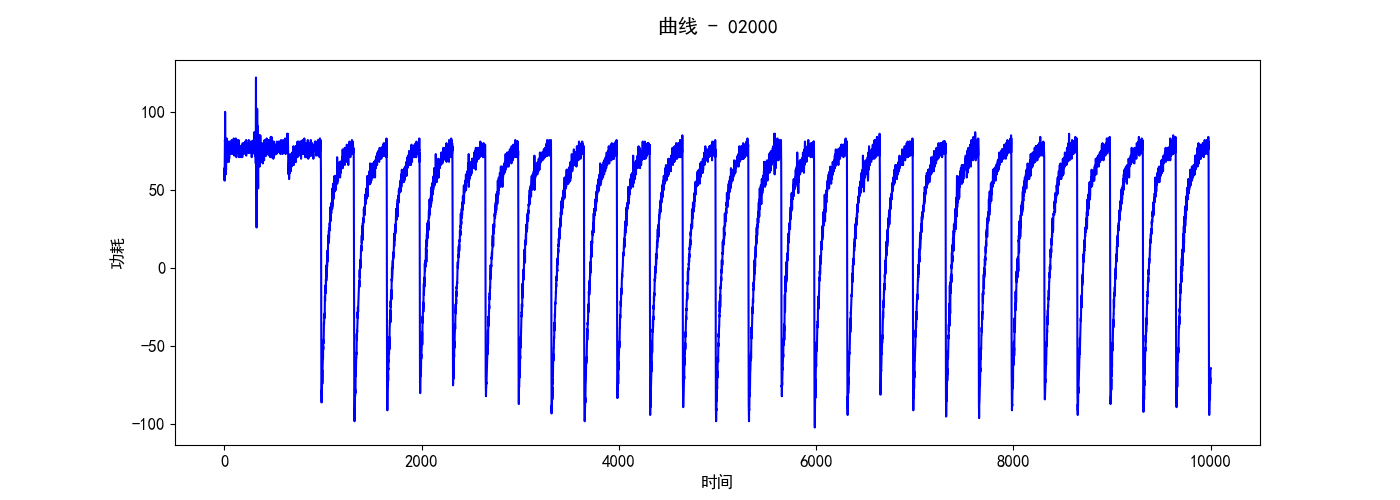
\includegraphics[height=.17\textheight, width=1.0\textwidth]{../images/trace_02000.png}
        % \caption{第 02000 条功耗曲线}
    \end{subfigure}
    \begin{subfigure}{1.0\textwidth}
        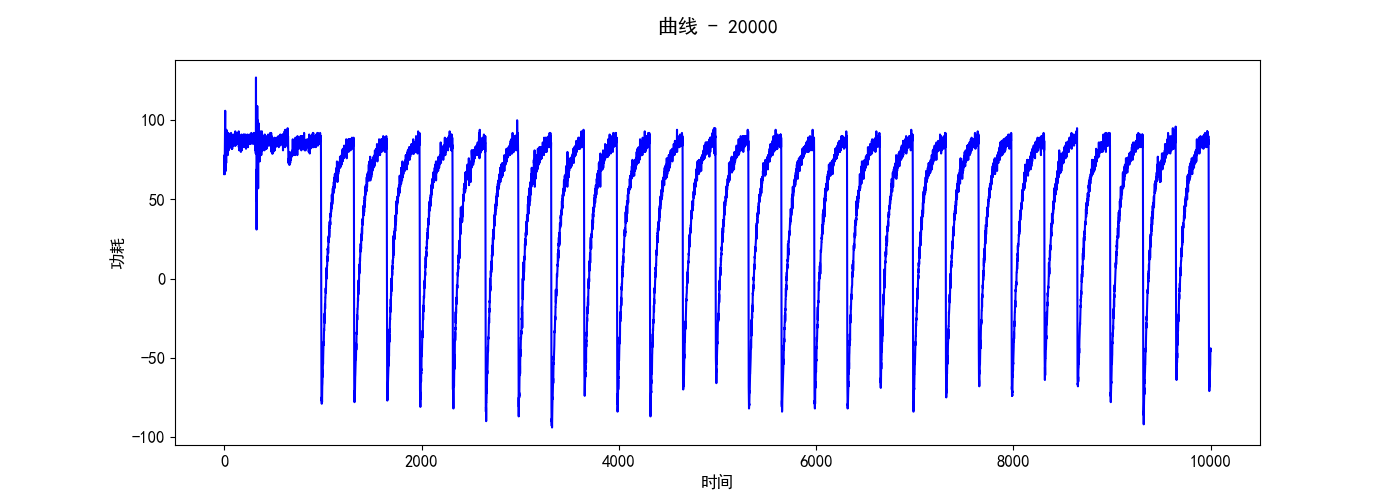
\includegraphics[height=.17\textheight, width=1.0\textwidth]{../images/trace_20000.png}
        % \caption{第 20000 条功耗曲线}
    \end{subfigure}

    \caption{ZUC 算法初始化阶段硬件电路的功耗曲线}

    \label{fig:traces}

\end{figure}

\newpage

\section{不同密钥猜测的相对相关系数}

按照在上一章中分析的流程,猜测不同的 k5 对应的中间值,总共有 256 种可能的情况。然后利用汉明重量模型,将其转换成假设功耗值,求解与实际功耗值之间的相关系数。由于选取的中间值在初始化阶段第一轮末尾,因此我们将攻击的部位选取为覆盖第一轮和第二轮的功耗点,因此实际参与计算的功耗点数在 500 左右。

我们将这些点上的相关系数求绝对值后,取最大的前 5 个值求平均,得到可以参考的平均相关系数。这样处理的目的是为了减小误差,防止某些无效的相关系数值遮盖了有效的值。为了和真正的“相关系数”作区分,我这里将其称为“相对相关系数”。

\vspace*{\baselineskip}

图 \ref{fig:keyguess} 展示了使用不同功耗曲线条数进行攻击,得到的 256 个密钥猜测的相对相关系数。横轴是密钥字节猜测的 10 进制值,纵轴是相对相关系数,绿色的虚线代表相对相关系数最高的猜测字节。

从图中可以得到这样一些信息:

\begin{enumerate}
    \item \textbf{当攻击的功耗曲线数目达到一定值之后,字节 171(AB)的相对相关系数保持最高。}\\
    因此 k5 最有可能是 171(AB)。而实验预设的密钥是“01 23 45 67 89 AB CD EF 01 23 45 67 89 AB CD EF”(k0 到 k15),k5 恰好是“AB”,这也就表明我们的最佳猜测是正确的,攻击成功。
    \item \textbf{在使用的功耗曲线条数为 100 时,根据相对相关系数猜测的最佳密钥字节是 43(2B),而这个猜测结果是错误的。}\\
    这表明当攻击使用的功耗曲线数目较少时,得到的结果可信度较低,这时最佳密钥字节猜测还不够稳定。因此在攻击时一定要测试猜测结果的稳定性,选用的方法就是使用更多的功耗曲线。\\
    一个值得注意的细节是,尽管猜测错误,但是“2B”对应的二进制值是“00101011”,和正确的“AB”对应的二进制值“10101011”仅仅相差一个比特。虽然不同字节在非线性变换后,输出的差异一般非常大,因此错误猜测和正确结果之间的关联一般没有参考价值,但是这里的细节可能表明,密码算法的非线性变换部分或许有微小的瑕疵,从而造成了某些不同的字节在输出后差异并没有想象中的那么大,攻击者有可能通过选择合适的明文,来扩大非线性变换中的漏洞,更高效地破解相关密钥字节。不过尚缺乏充分的实验来证明这一猜想。
    \item \textbf{当使用的功耗曲线条数越来越多时,正确的密钥字节对应的相对相关系数明显高于错误的密钥字节。}\\
    这个现象的原因是显然的,随着功耗曲线条数的增多,错误密钥字节产生的中间值与正确密钥字节产生的中间值差异愈发明显,偶然性渐渐被必然性覆盖。因此,选用尽可能多的功耗曲线条数,一般可以提高攻击的成功率。
    \item \textbf{随着功耗曲线条数的增多,相对相关系数的最大值呈减小趋势。}\\
    比如使用的功耗曲线条数为 1000 时,最高相对相关系数约为 0.25,而当使用的功耗曲线条数到 20000 时,最高相对相关系数已经降低到大概 0.15 了。事实上,不仅最高相对相关系数在减小,所有密钥字节猜测对应的相对相关系数,整体上都在减小。这是因为,尽管假设功耗值(依据理论中间值和功耗模型计算得到)和实际功耗值之间存在一定的联系,但这种联系不一定是强正相关的。所以当攻击采用的功耗曲线条数很多时,假设功耗值与实际功耗值之间不相关的部分占比就会变大。\\
    为什么假设功耗值与理论功耗值有不相关的地方呢?直观的原因是,电路执行某个操作的时间并不是每一次都完全对齐的,或者某些频率的噪声对曲线的波形产生了影响。还有一些更底层更根本的原因,比如选取的功耗模型并不能真正反映实际的功耗值大小,我们此次采用的汉明重量模型,是基于“设备的功耗和操作的数据中的 1 的个数有关”这一假设,而事实可能并非如此:设备的功耗可能不仅仅和数据中 1 的个数有关,既可能和数据中 0 的个数有关,也可能和从 0 到 1 或者从 1 到 0 的比特数目有关,而且设备的功耗也不完全取决于操作的数据,还可能和控制命令也有关系,或者操作相关数据的同时,还可能在运行其他的指令、操作其他不相关的数据。\\
    既然这样,那么为什么本次实验中,功耗曲线条数越多,正确密钥猜测的相对相关系数越突出呢?这是因为,正确密钥字节对应的假设功耗值和实际功耗值中相关的部分比例高于不相关部分的比例。功耗曲线数目的增加并不会改变这种比例,因此尽管整体上相关系数的绝对数值降低了,但是正确的密钥字节对应的假设功耗值仍旧比错误的密钥字节更接近于实际功耗值。\\
    因此,尽管随着功耗曲线条数的增加,整体的相对相关系数的数值存在减小趋势,但是这也降低了偶然因素的影响,使得正确密钥字节对应的假设功耗值与实际功耗值之间的关联度,更加稳定地优于错误的密钥猜测。


\end{enumerate}

\begin{figure}[htbp]
    \centering

    \begin{subfigure}{1.0\textwidth}
        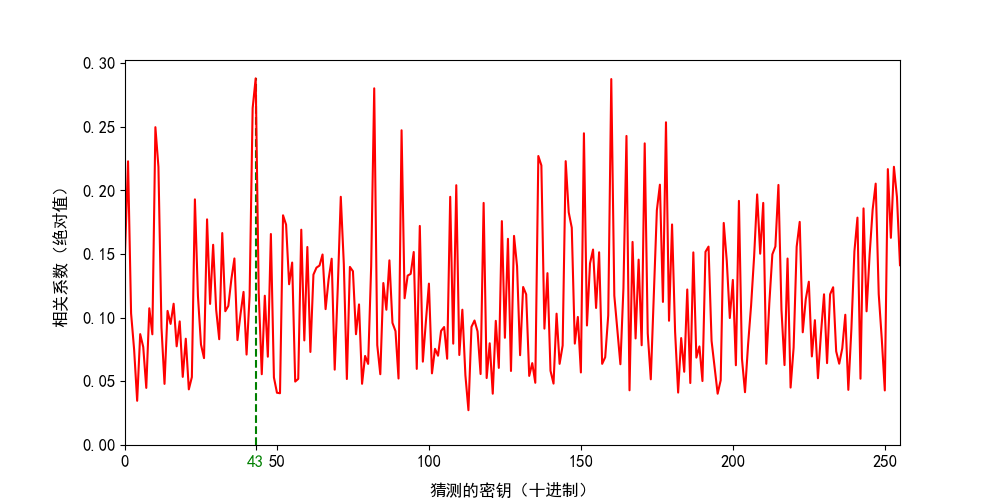
\includegraphics[height=.21\textheight, width=1.0\textwidth]{../images/keyguess_100.png}
        \caption{攻击使用的功耗曲线条数:100}
    \end{subfigure}
    \begin{subfigure}{1.0\textwidth}
        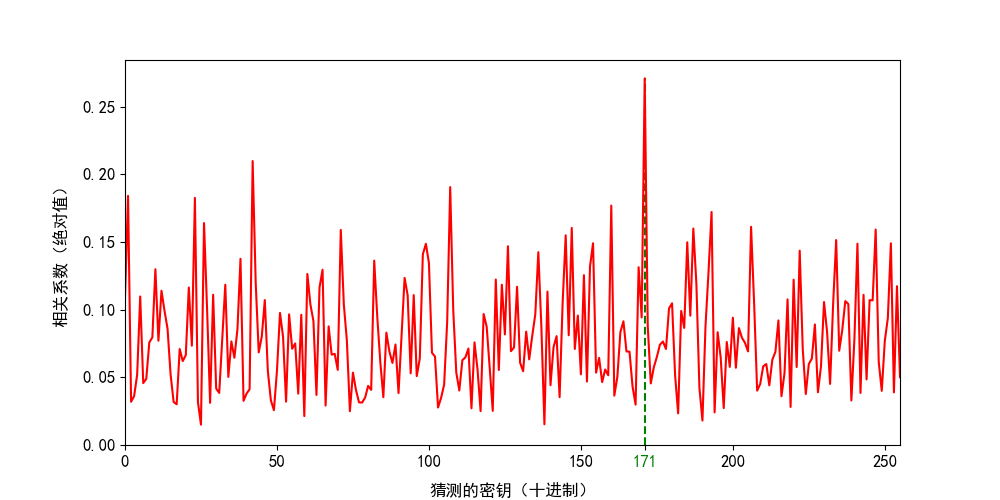
\includegraphics[height=.21\textheight, width=1.0\textwidth]{../images/keyguess_200.png}
        \caption{攻击使用的功耗曲线条数:200}
    \end{subfigure}
    \begin{subfigure}{1.0\textwidth}
        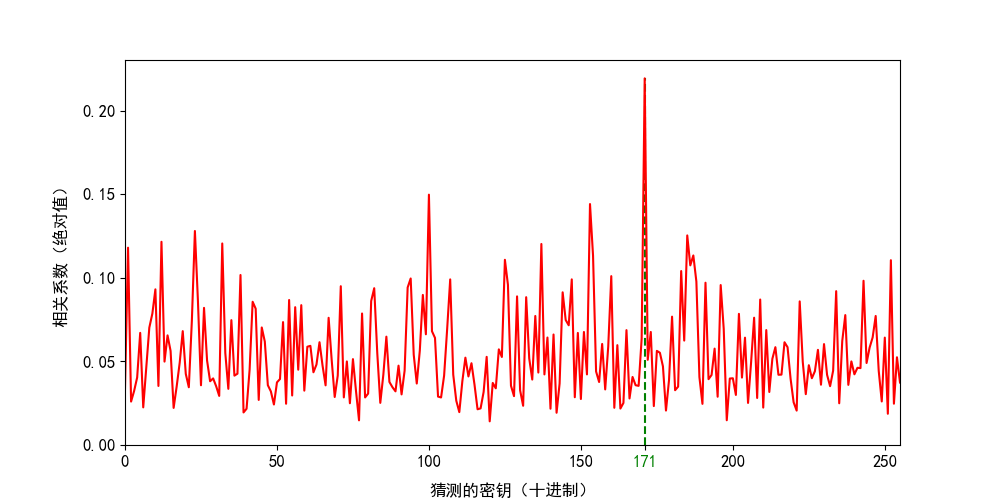
\includegraphics[height=.21\textheight, width=1.0\textwidth]{../images/keyguess_500.png}
        \caption{攻击使用的功耗曲线条数:500}
    \end{subfigure}
    \begin{subfigure}{1.0\textwidth}
        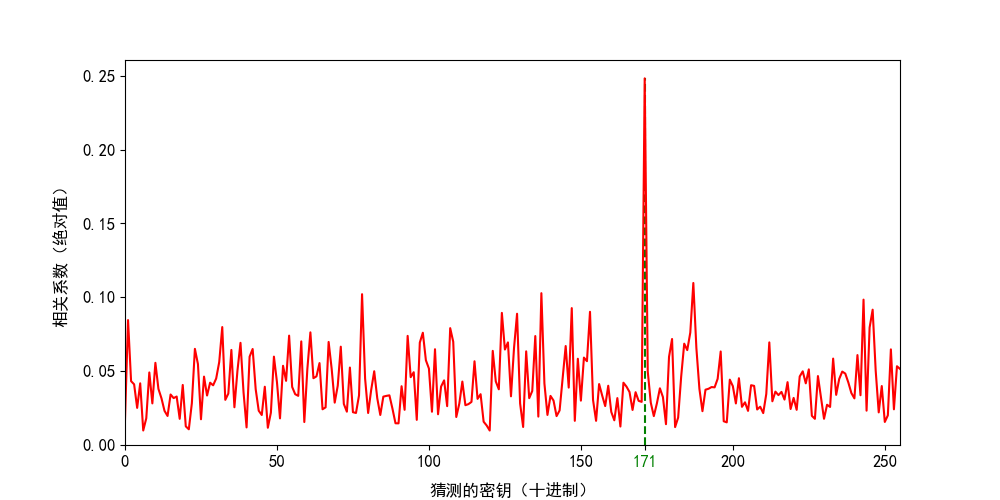
\includegraphics[height=.21\textheight, width=1.0\textwidth]{../images/keyguess_1000.png}
        \caption{攻击使用的功耗曲线条数:1000}
    \end{subfigure}
    \caption{使用不同功耗曲线条数进行攻击,得到 256 个密钥猜测的相对相关系数(1)}
    \label{fig:keyguess}
\end{figure}
 
\begin{figure}[htbp]
\ContinuedFloat
    \begin{subfigure}{1.0\textwidth}
        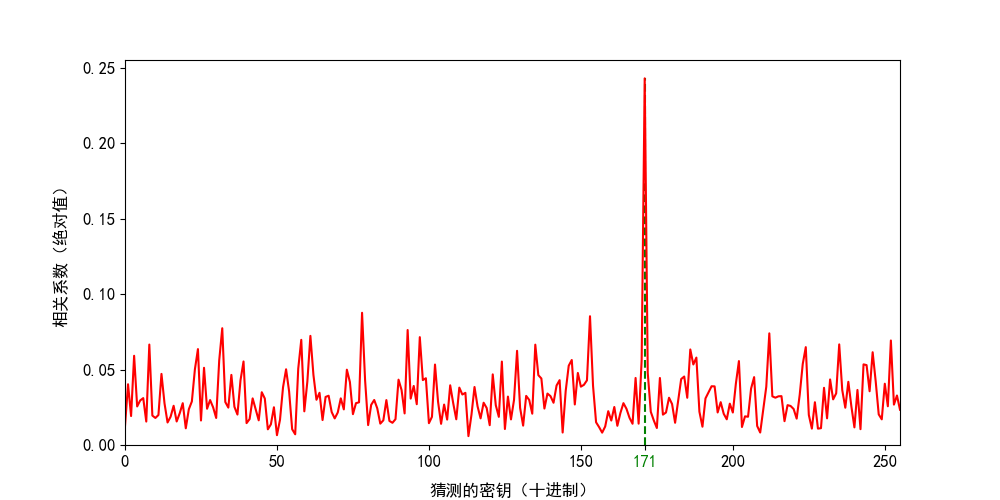
\includegraphics[height=.21\textheight, width=1.0\textwidth]{../images/keyguess_2000.png}
        \caption{攻击使用的功耗曲线条数:2000}
    \end{subfigure}
    \begin{subfigure}{1.0\textwidth}
        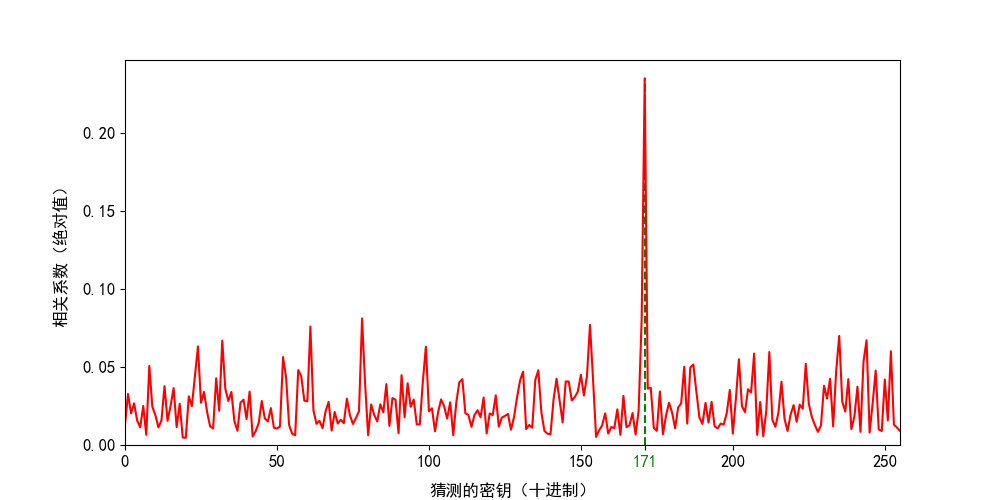
\includegraphics[height=.21\textheight, width=1.0\textwidth]{../images/keyguess_5000.png}
        \caption{攻击使用的功耗曲线条数:5000}
    \end{subfigure}
    \begin{subfigure}{1.0\textwidth}
        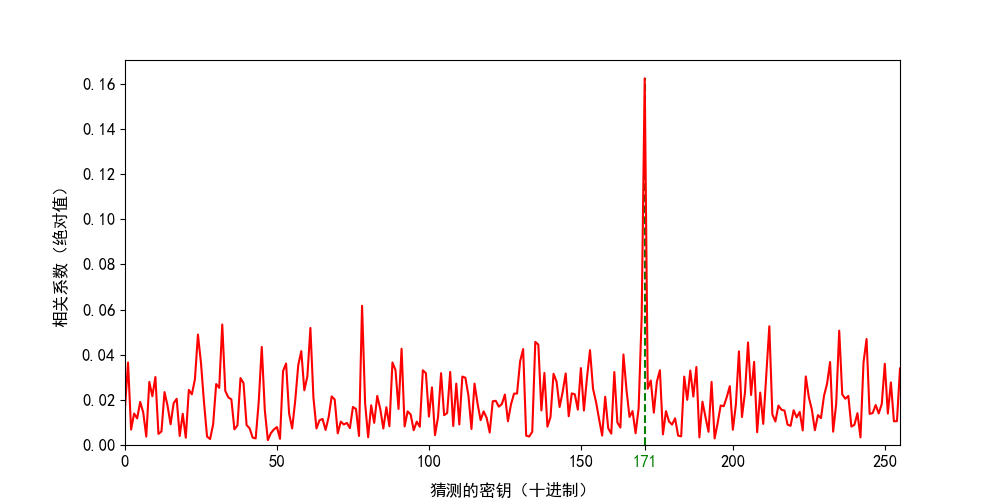
\includegraphics[height=.21\textheight, width=1.0\textwidth]{../images/keyguess_10000.png}
        \caption{攻击使用的功耗曲线条数:10000}
    \end{subfigure}
    \begin{subfigure}{1.0\textwidth}
        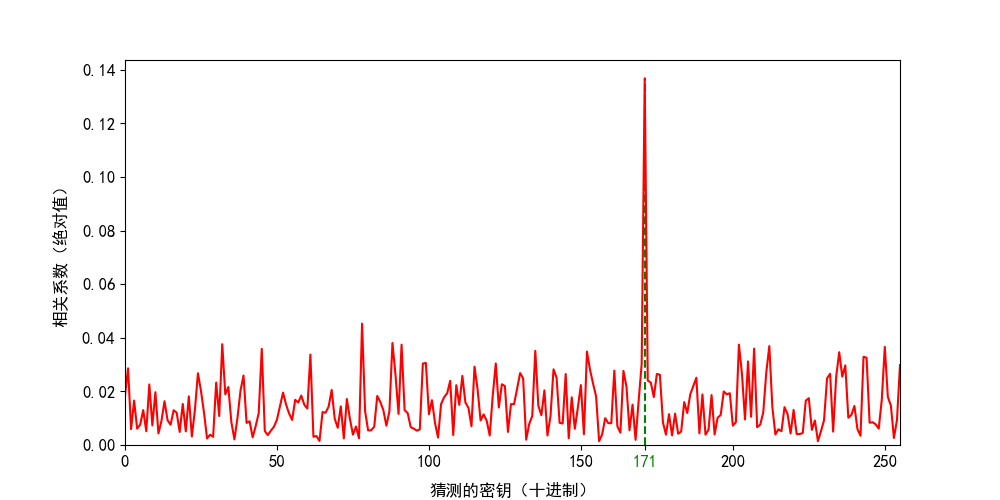
\includegraphics[height=.21\textheight, width=1.0\textwidth]{../images/keyguess_20000.png}
        \caption{攻击使用的功耗曲线条数:20000}
    \end{subfigure}

    \caption{使用不同功耗曲线条数进行攻击,得到 256 个密钥猜测的相对相关系数(2)}
    % \label{fig:keyguess}
\end{figure}

\newpage

\section{功耗曲线条数对相关系数的影响}

上一节中从侧面反映了不同猜测密钥字节的相对相关系数和功耗曲线条数的关系,这一小节将更加完整地展现二者之间的联系。

\vspace*{\baselineskip}

图 \ref{fig:keyrank} 展示了不同密钥猜测的相对相关系数随功耗曲线条数变化情况。图中不同颜色的线代表不同的密钥猜测。图 \ref{fig:keyrank_2000} 和 图 \ref{fig:keyrank_20000} 中相对相关系数最高的曲线对应的密钥字节为 171(AB),也即正确的密钥字节。

从图中可以得到这样一些信息:

\begin{enumerate}
    \item \textbf{攻击使用的功耗曲线条数较少时,无法分析出正确的密钥字节。}这一点已经在上一节详细阐述过,不再赘述。
    \item \textbf{当攻击使用的功耗曲线条数超过一定值时,能够稳定地分析出正确的密钥字节。}这一点也已经在上一节详细阐述过,不再赘述。
    \item \textbf{在攻击使用的曲线条数到达 5000 和 17500 左右时,相对相关系数的值均出现了明显的下降。}\\
    相对相关系数整体随着功耗曲线条数的增加而减小的原因,已经在上一节讨论过了,但是这里关注的问题是,为什么在这两个节点出现了相对相关系数的剧烈下降?而且不单是正确的密钥字节,所有密钥猜测的相对相关系数都同时出现陡降。一个合理的解释是,在这两个节点,采集的功耗曲线出现了在时间上微弱的偏移,导致后面的曲线组与前面曲线组不对齐。由于相对系数的计算和所有的功耗曲线都相关,因此如果后面采集的功耗曲线与前面的不完全对齐,就有可能造成攻击效果下降。
    \item \textbf{在攻击使用的曲线条数从 5000 到 17500 的区间内,相对相关系数的值出现了缓慢的爬升。}\\
    这一现象与上一点并不矛盾,反而是支持功耗曲线出现时间偏移的有力证据。相对相关系数在第 5000 条到 17500 条这一段中出现了爬升,一个合理的解释是,尽管这一段曲线与 第 1 到 5000 条是不对齐的,但是段内的曲线是对齐的,因此分析这一段时间内采集到的曲线,会渐渐不足之前不对齐造成的影响,因而出现相对相关系数的缓慢爬升。

\end{enumerate}

\begin{figure}[htbp]
    \centering

    \begin{subfigure}{1.0\textwidth}
        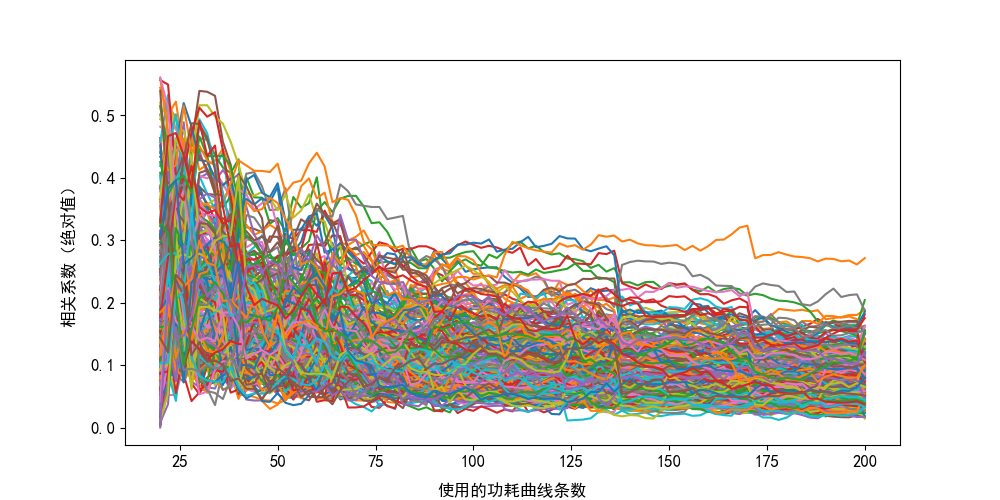
\includegraphics[height=.25\textheight, width=1.0\textwidth]{../images/keyrank_200_2.png}
        \caption{攻击使用的功耗曲线条数变化范围:20 -- 200}
    \end{subfigure}

    \begin{subfigure}{1.0\textwidth}
        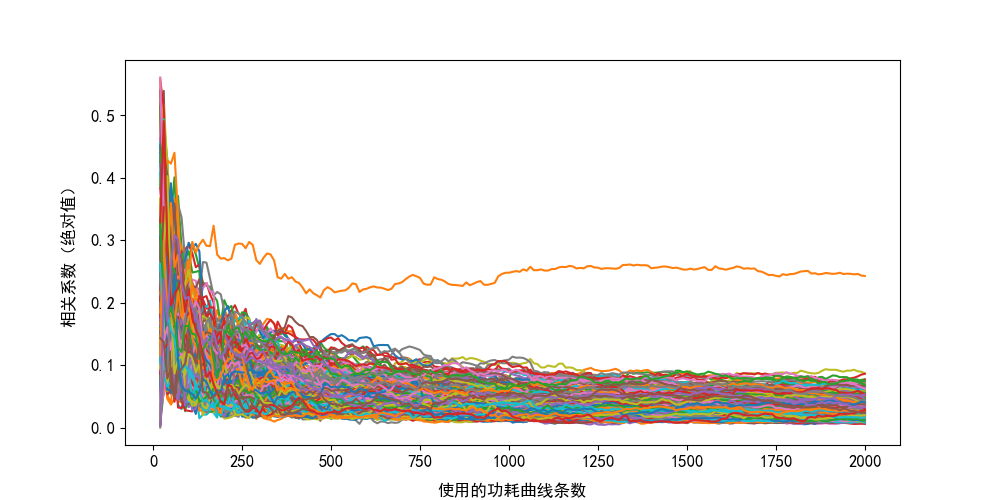
\includegraphics[height=.25\textheight, width=1.0\textwidth]{../images/keyrank_2000_10.png}
        \caption{攻击使用的功耗曲线条数变化范围:20 -- 2000}
        \label{fig:keyrank_2000}
    \end{subfigure}

    \begin{subfigure}{1.0\textwidth}
        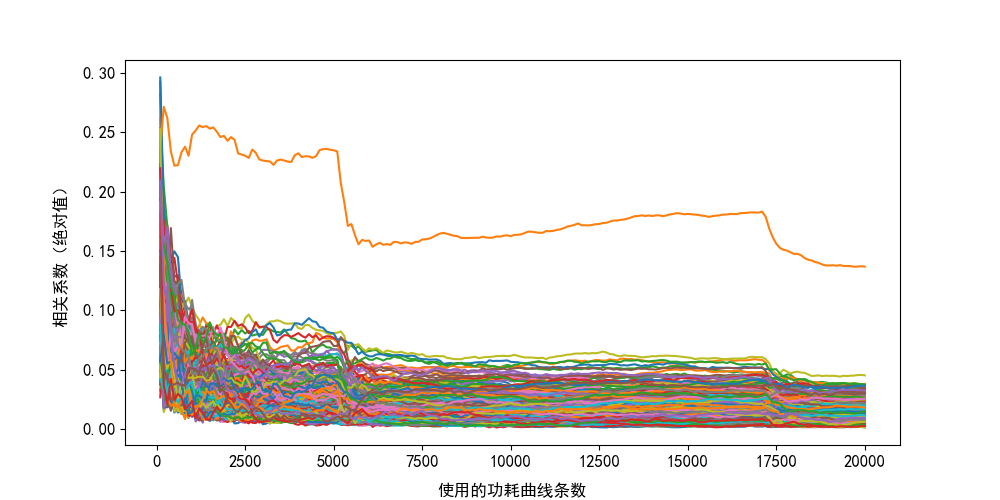
\includegraphics[height=.25\textheight, width=1.0\textwidth]{../images/keyrank_20000_100.png}
        \caption{攻击使用的功耗曲线条数变化范围:20 -- 20000}
        \label{fig:keyrank_20000}
    \end{subfigure}

    \caption{不同密钥猜测的相对相关系数随功耗曲线条数变化情况}
    \label{fig:keyrank}
\end{figure}

\newpage

\section{密钥信息的泄露位置}

尽管我们之前已经从理论上推测密钥信息泄露的位置应该在初始化阶段第一轮末尾,但是我们在攻击时是取覆盖第一轮和第二轮的一段区间的。如果我们想得到泄露密钥信息的更精确的位置,就需要计算正确密钥字节产生的中间值,然后计算出假设功耗值,求出其与实际功耗值的相关系数。从相关系数的变化中就能看出密钥信息的泄露位置。

\vspace*{\baselineskip}

图 \ref{fig:leakage} 展示了密钥字节 k5 的功耗信息泄露情况。图 \ref{fig:leakage_zoom} 则将泄露位置放大,以进行更加细致的观察。

从图中可以得到如下信息:

\begin{enumerate}
    \item \textbf{攻击使用的功耗曲线条数较少时(100 条),密钥字节几乎无泄露。}
    \item \textbf{攻击使用的功耗曲线超过 200 条时,就已经出现了较为明显的泄露。}
    \item \textbf{随着攻击使用的功耗曲线条数的增加,对应位置功耗泄露的情况越发明显。}
    \item \textbf{泄露的位置在初始化阶段第一轮的末尾和第二轮的开始之间。}
\end{enumerate}

\vspace*{\baselineskip}

这些结论都是显而易见的,原因也都在上面的结果中分析过了,因此这里不再重复。

\vspace*{\baselineskip}

既然找到了泄露的位置,下一步的工作就是要对该部分进行防护了。由于算法本身不能修改,因此可以做的就是在硬件实现上进行改进。由于泄露的中间值是由于 S 盒的非线性变换引起的,因此可以对 S 盒做一些防护措施,比如最常用的就是加入掩码。不过这超出了本次实验的内容,可以留到今后进行更加深入的研究和分析。


\begin{figure}[htbp]
    \centering

    \begin{subfigure}{1.0\textwidth}
        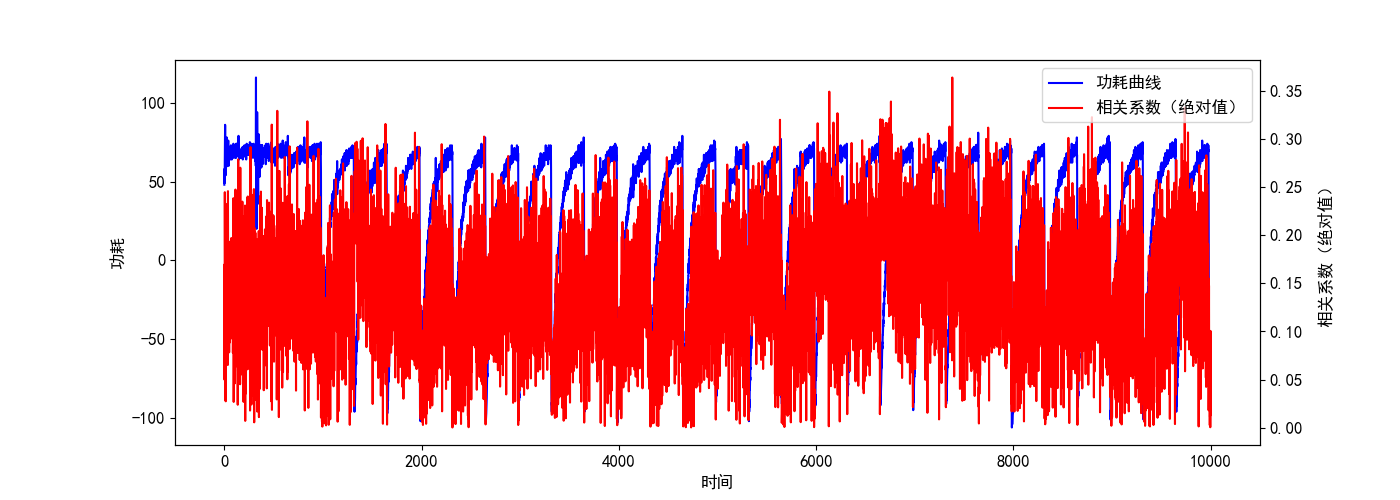
\includegraphics[height=.21\textheight, width=1.0\textwidth]{../images/leakage_100.png}
        \caption{攻击使用的功耗曲线条数:100}
    \end{subfigure}
    \begin{subfigure}{1.0\textwidth}
        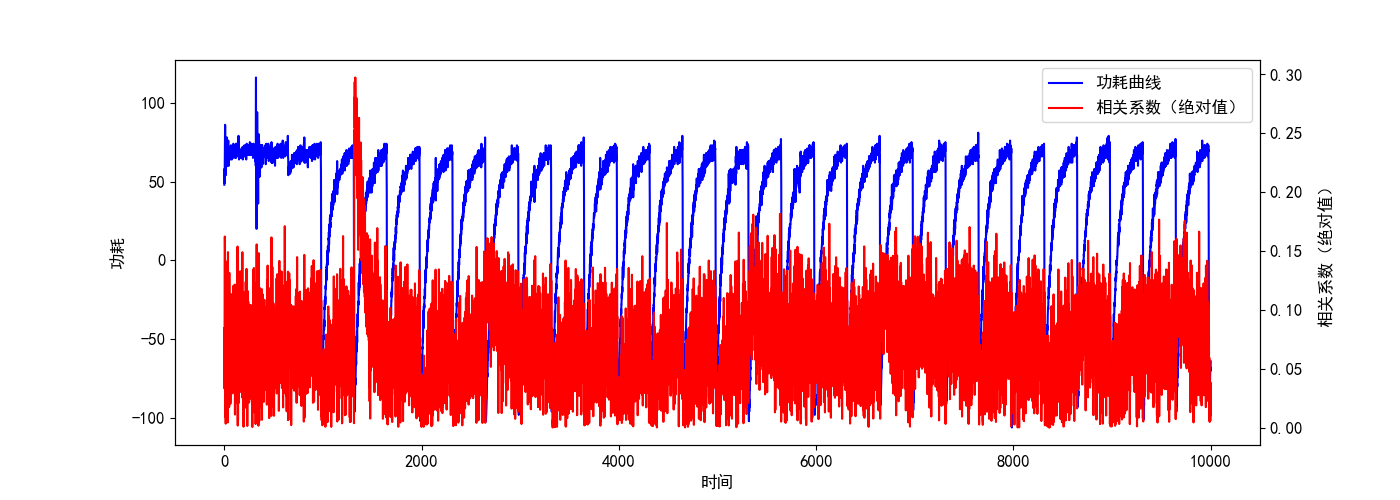
\includegraphics[height=.21\textheight, width=1.0\textwidth]{../images/leakage_200.png}
        \caption{攻击使用的功耗曲线条数:200}
    \end{subfigure}
    \begin{subfigure}{1.0\textwidth}
        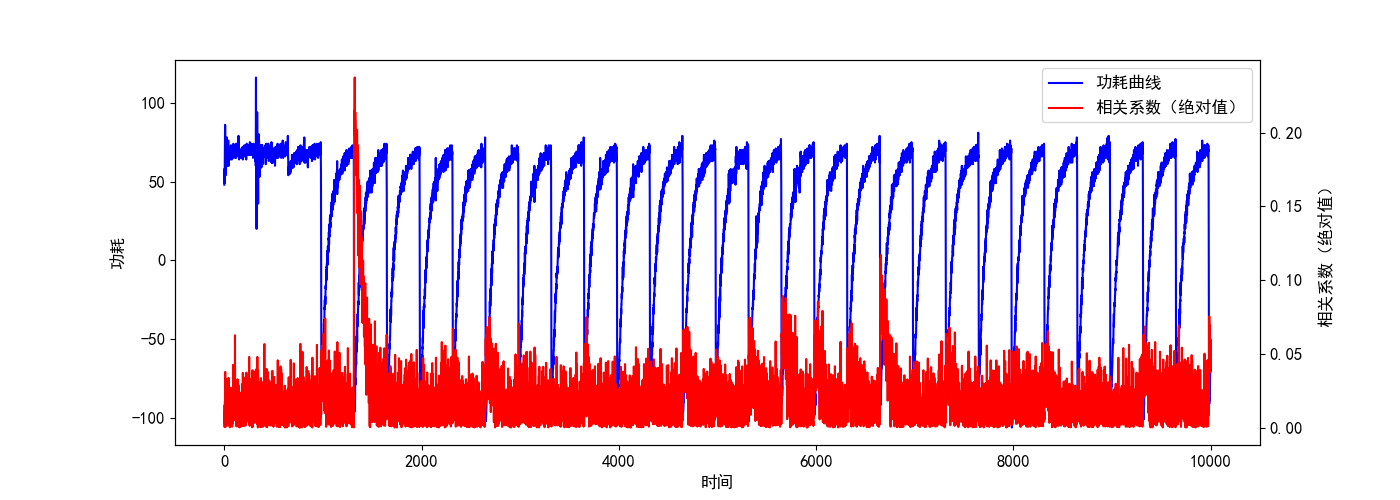
\includegraphics[height=.21\textheight, width=1.0\textwidth]{../images/leakage_500.png}
        \caption{攻击使用的功耗曲线条数:500}
    \end{subfigure}
    \begin{subfigure}{1.0\textwidth}
        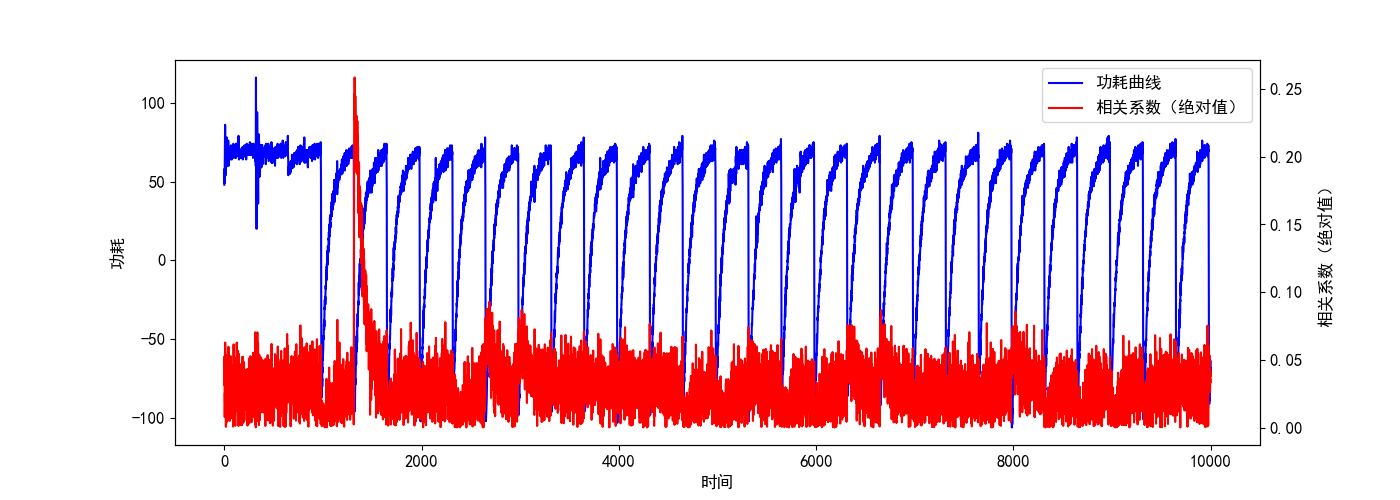
\includegraphics[height=.21\textheight, width=1.0\textwidth]{../images/leakage_1000.png}
        \caption{攻击使用的功耗曲线条数:1000}
    \end{subfigure}

    \caption{正确密钥字节对应的假设功耗值与实际功耗值的相关系数(1)}
    \label{fig:leakage}
\end{figure}

\begin{figure}[htbp]
\ContinuedFloat
    \begin{subfigure}{1.0\textwidth}
        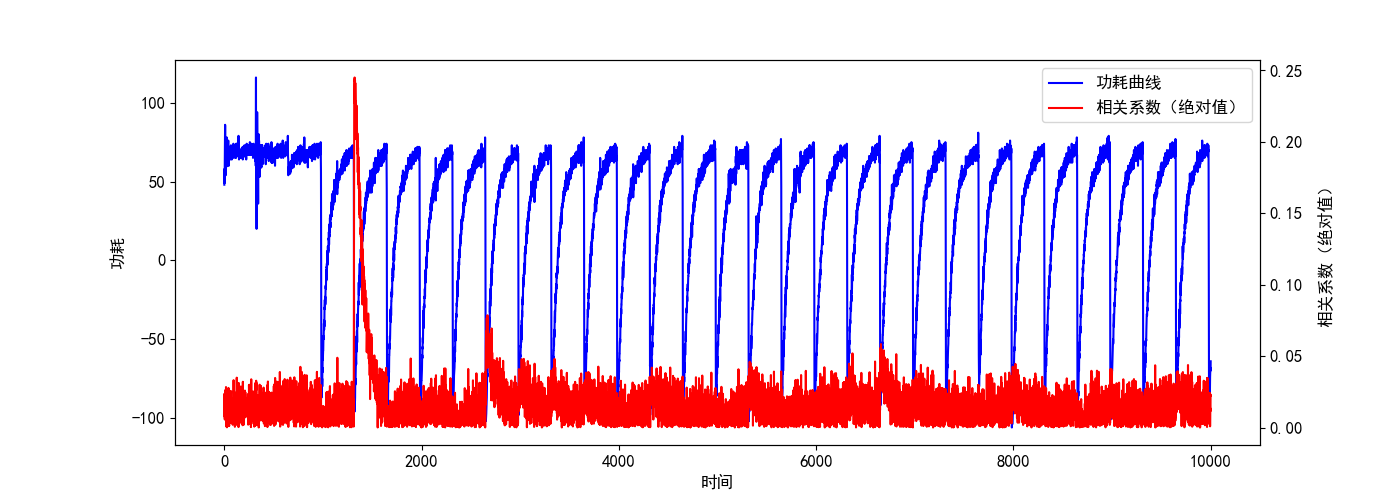
\includegraphics[height=.21\textheight, width=1.0\textwidth]{../images/leakage_2000.png}
        \caption{攻击使用的功耗曲线条数:2000}
    \end{subfigure}
    \begin{subfigure}{1.0\textwidth}
        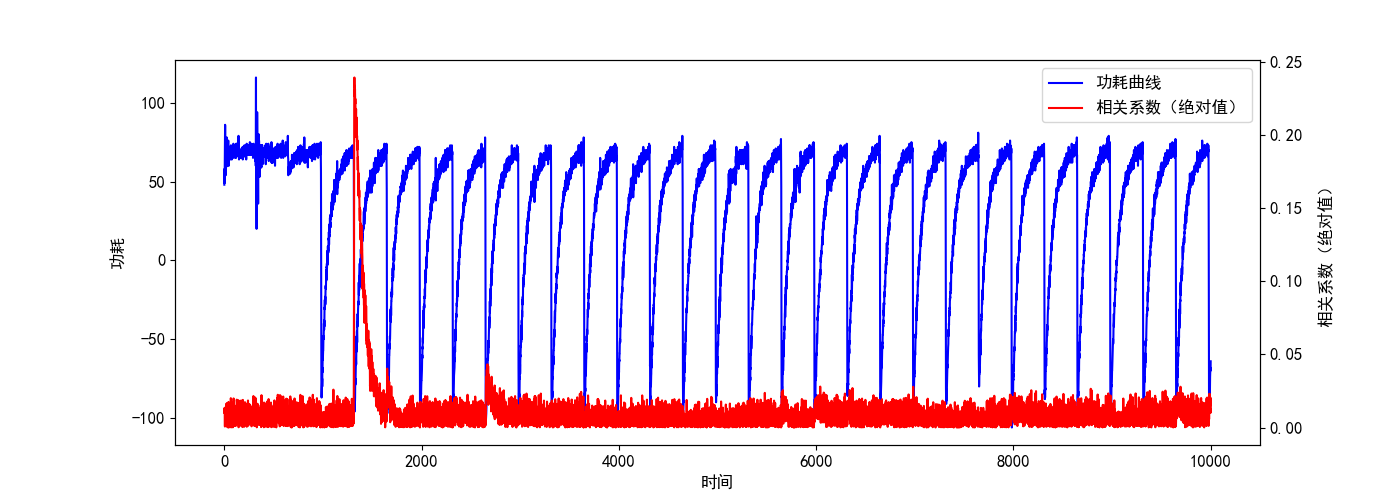
\includegraphics[height=.21\textheight, width=1.0\textwidth]{../images/leakage_5000.png}
        \caption{攻击使用的功耗曲线条数:5000}
    \end{subfigure}
    \begin{subfigure}{1.0\textwidth}
        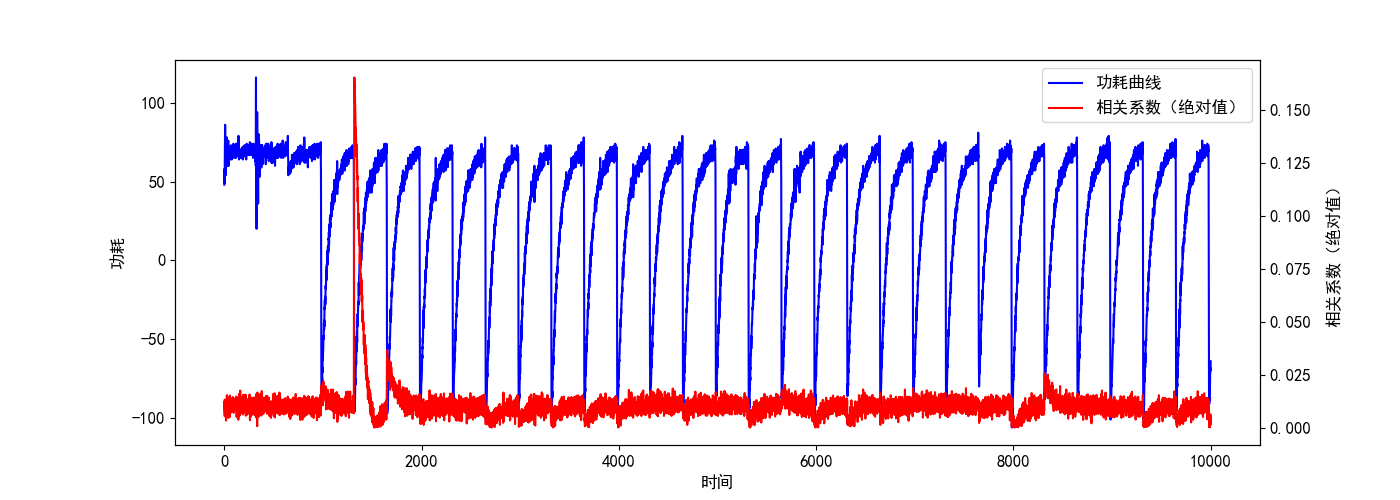
\includegraphics[height=.21\textheight, width=1.0\textwidth]{../images/leakage_10000.png}
        \caption{攻击使用的功耗曲线条数:10000}
    \end{subfigure}
    \begin{subfigure}{1.0\textwidth}
        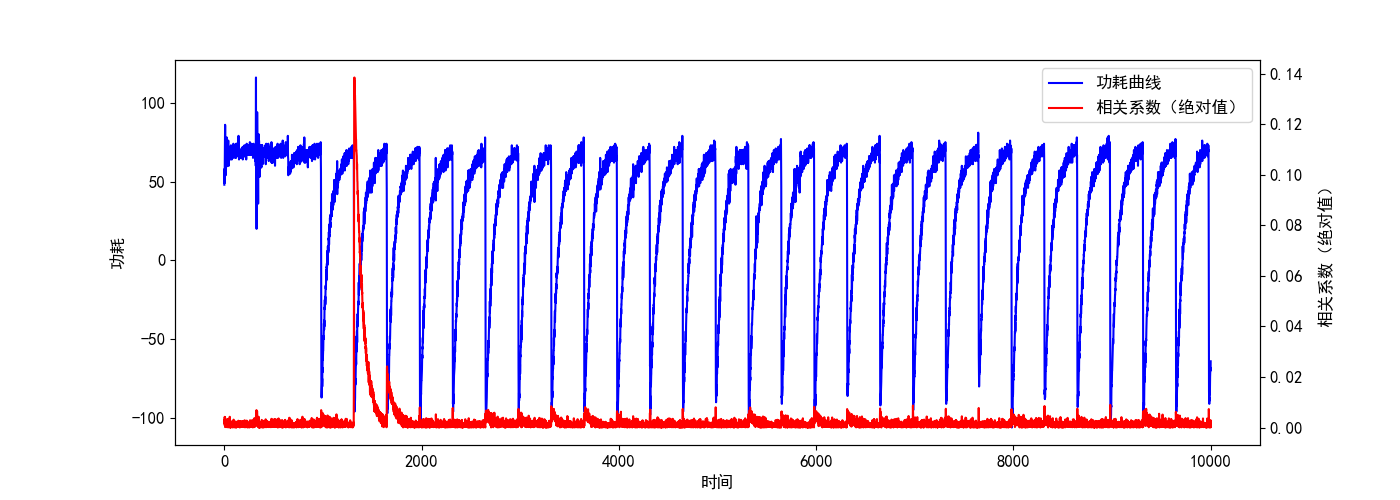
\includegraphics[height=.21\textheight, width=1.0\textwidth]{../images/leakage_20000.png}
        \caption{攻击使用的功耗曲线条数:20000}
    \end{subfigure}

    \caption{正确密钥字节对应的假设功耗值与实际功耗值的相关系数(2)}
    % \label{fig:leakage}
\end{figure}

\begin{figure}[htbp]
    \centering
    \begin{subfigure}{1.0\textwidth}
        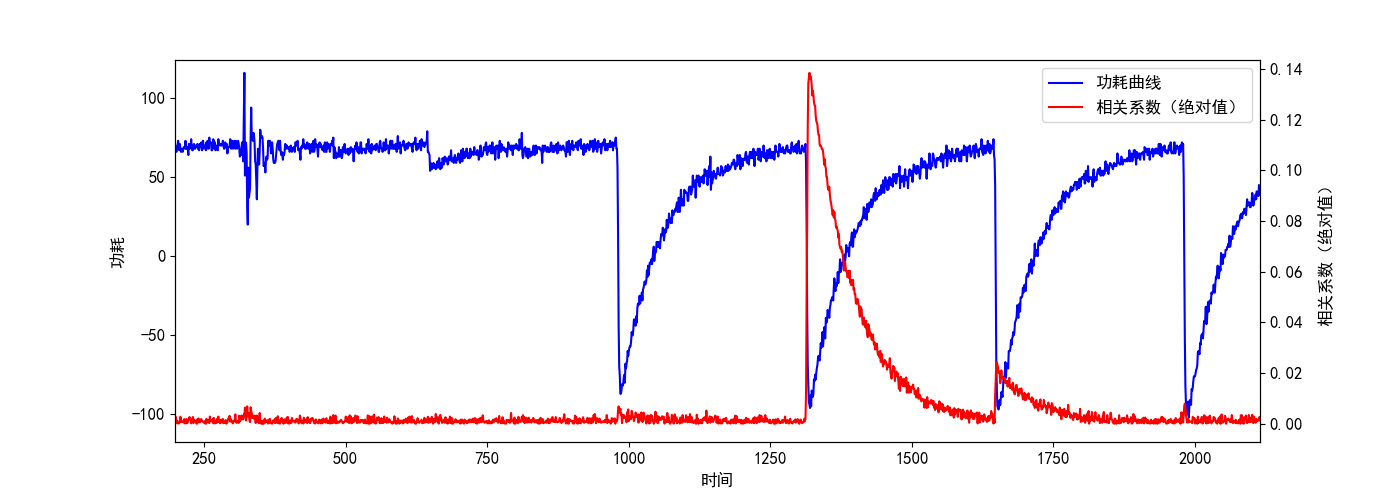
\includegraphics[height=.25\textheight, width=1.0\textwidth]{../images/leakage_20000_zoom_1.png}
        \caption{使用 20000 条功耗曲线时的泄露情况(放大 5 倍)}
    \end{subfigure}
    \begin{subfigure}{1.0\textwidth}
        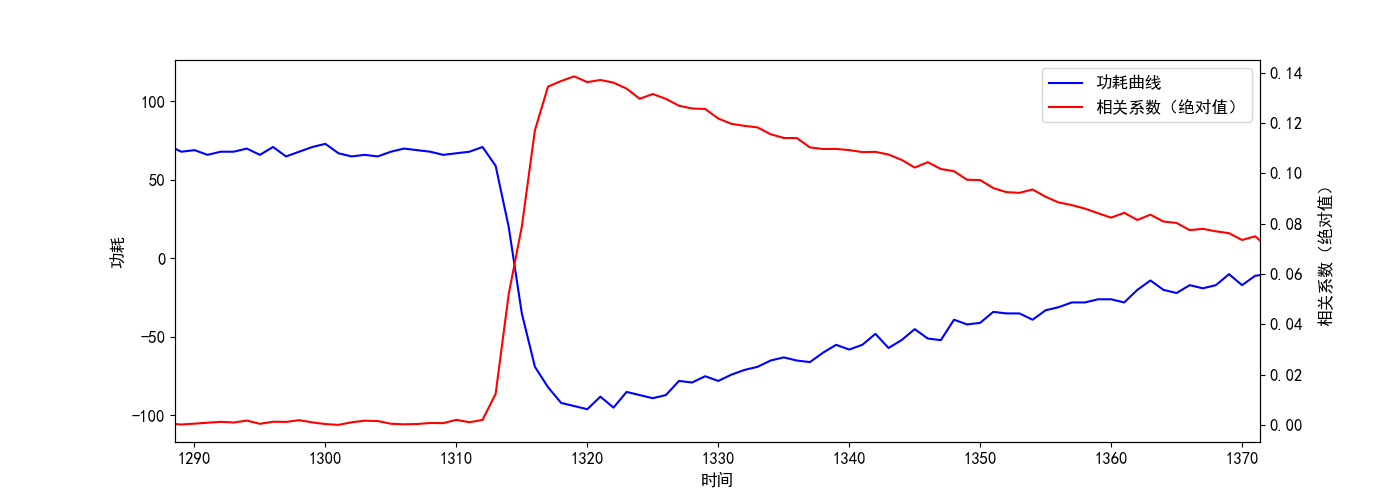
\includegraphics[height=.25\textheight, width=1.0\textwidth]{../images/leakage_20000_zoom_2.png}
        \caption{使用 20000 条功耗曲线时的泄露情况(放大 140 倍)}
    \end{subfigure}

    \caption{密钥字节功耗泄露情况的细节(使用 20000 条功耗曲线)}
    \label{fig:leakage_zoom}
\end{figure}


\section{本章小结}

本章首先展示了 ZUC 算法电路实际运行时采集的功耗曲线,简单分析了功耗曲线的特征,推测出了一些基本的信息。

然后我们对采集到的功耗曲线实施了差分功耗分析攻击,得到了不同密钥猜测对应的相对相关系数。实验结果表明我们的攻击是成功的,得到了正确的密钥字节。与此同时,我们还发现了相对相关系数和功耗曲线条数有关的现象。

接着我们讨论了攻击使用的功耗曲线条数对相关系数的影响,指出了相对相关系数随功耗曲线条数增加时出现的变化,并且根据事实和观察给出了可能的原因和合理的解释。

最后我们分析了密钥信息的泄露位置,发现功耗泄露的位置确实是理论分析得到的地方,说明我们的思路和方法是正确的。